

In this chapter a short overview on the basic concepts of Convolutional Neural Networks (CNNs) will be given. 
The scope is to give the necessary background for the understanding of the structure and the motivations behind the 
Deep Learning (DL) models employed for the analysis of BCDI data, presented in the next chapters.  

For more comprehensive and exhaustive dissertations about Machine Learning (ML) and Artificial Neural Networks (ANNs)
the book of Goodfellow \cite{Goodfellow_2016} and the more recent from Prince \cite{prince2023understanding} are 
suggested to the reader. 

\section{Artificial Neural Networks (ANNs)}

ANNs is a type of machine learning algorithm inspired by the biological neuron structure. ANNs are generally composed of interconnected 
nodes where the signal is processed through operations with tunable parameters named weights 
and biases for multiplications and addition respectively. Important feature of each node is the \textit{activation function}, 
that introduces a non-linear operation and returns the node's output \cite{jagtap2022}. Several kinds of these 
activation functions exist and their use depends on the properties of each (bounds, derivatives, positivity, etc.) 
\cite{kunc2024}. In the following chapters the modified rectifying linear unit, known as LeakyReLU \cite{Maas2013RectifierNI}, 
and the sigmoid, also known as logistic, function will be used. Neurons are generally organized into \textit{layers} and 
are connected between neurons of other layers. In \textit{feed-forward} neural networks the information flows from the 
input layer to the output layer with forward connections only.
In other neural networks, like \textit{recurrent} ones, the connections are also designed backwards. 

\begin{figure}[H]
    \centering
    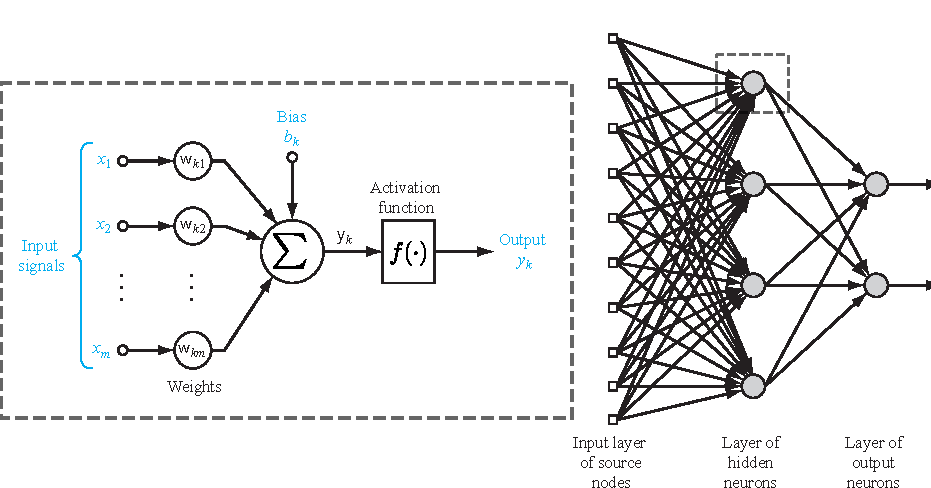
\includegraphics[width=\textwidth]{figures/Intro/neuron2.pdf}
    \caption{\textbf{Schematic of an artificial neuron and a neural network.} On the left, a series of input signals 
    $x_i$ are multiplied by the tunable weight $w_{k}$ and summed together with the tunable bias $b_k$ relative to 
    the $k$-th neuron. The output is then passed through the activation function $f$ which produce an output $y_k$ 
    which is a non-linear combination of the inputs. On the right, the feed-forward network composed 
    of two \textit{hidden} layers of artificial neurons processing the ten units long vector $x$ and returning a 
    binary output. Networks of this type are said to be \textit{fully connected} as each input component, or 
    node's output is processed by all neurons. Adapted from \cite{haykin2009neural}}
    \label{fig:neuron}
\end{figure}

\subsection{Neural networks as universal approximators}

The use of non-linear functions is found to be fundamental for the powerful analytical and statistical properties of ANNs, 
which have been progressively 
established over the years. It was shown \cite{Cybenko1989, Hornik_1989, Leshno_1993} that ANNs with appropriate 
activation functions and sufficient parameters can approximate \textit{any} continuous function on a compact domain to arbitrary 
accuracy (\textit{universal approximation theorems}). Later the proof has been extended to deep convolutional neural 
networks as well \cite{UniversalityCNN_2020}.

Formally, we can consider $\mathcal{X}$ as the set of all events belonging to the same statistical distribution and 
$\mathcal{Y}$ similarly. We also assume that an unknown mapping $\mathcal{M}$ between an input $x \in \mathcal{X}$ and the output 
$y = \mathcal{M}(x)$ exists. At this point, the goal of the ANNs is to be the closest approximation of $\mathcal{M}$.
Typically, this implies seeking the combination of parameters $\theta_k = (w_k, b_k)$ of the neural network $\mathcal{N}_{\theta}$ 
such that $\mathcal{N}_{\theta} \approx \mathcal{M}$

\textbf{How is this mapping found?} The core idea is known as Empirical Risk Minimization and states that 
when the $\theta_k$ are adjusted to fit a sufficiently large dataset consisting of samples drawn from an underlying distribution, 
the function being approximated reflects the statistical relationships encoded in that distribution \cite{Hornik_1990}.
By the Law of Large Numbers, the empirical distribution observed in the \textit{training set} converges to the true 
distribution as the sample size grows, and thus the empirical risk minimized during training approaches the true 
risk. This statistical foundation explains why ANNs are able to generalize to new, unseen data drawn from the 
same population. 

It is therefore sufficient to have a large but finite number of samples representative of both the sets $\mathcal{X}$ 
and $\mathcal{Y}$ to approximate $\mathcal{M}$. This powerful statistical property underlies the concept of \textit{supervised} 
training of ANNs. 

More formally, one can consider having a limited set of $N$ examples $(x_1,y_1 = \mathcal{M}(x_1)), ..., (x_N, y_N = \mathcal{M}(x_N))$ 
which we call \textit{training set} $\mathcal{T}$. Here, each $x_i$ is an input instance and $y_i$ the 
corresponding ground truth transformation operated by $\mathcal{M}$. We can now introduce a non-negative scalar 
real-valued \textit{loss function} $L(\hat{y},y )$ which measures the difference between the ground truth $y$ and the 
output of the neural network $\hat{y} = \mathcal{N}_\theta (x)$ for each element of the training set.

It follows that the best approximation of the mapping $ \mathcal{N}_\theta^{\mathcal{T}} \approx \mathcal{M}^{\mathcal{T}}$ is 
obtained when the score of the loss function averaged across the number of training samples is lowest.
The problem of approximating the mapping between the input and ground truth in the training set is then formulated as 
minimization problem of the type: 

\begin{equation}
    \hat{\theta}_{\mathcal T}
    = \arg\min_{\theta} 
    \left\{ \frac{1}{N} \sum_{i=1}^N 
    L\!\left(y_i, \mathcal{N}_{\theta}^{\mathcal{T}}(x_i)\right) 
    \right\}
\end{equation}

For a sufficiently large $N$ the $\hat{\theta}_{\mathcal T} \approx \hat{\theta}$ valid for the whole statistical distribution. 
The size of $N$ needed to approach the true mapping depends obviously on the complexity of the mapping and on the 
complexity of the minimization task. While the first is inherent to the problem, the second can be engineered with 
the choice of a metric for which the loss function minimization is easier. This will be clear in Chapter \ref{chap:phase_retrieval}
where different loss functions are tested. In the same way, the network design can impact the facility with which the 
ANN converges to the approximation of the desired mapping. In these regards, the use of multiple intermediate layers 
of neurons (\textit{hidden layers}) was shown to strongly improve the ability of the NN to fit more complex functions
(see \cite{prince2023understanding} - Chapter 4.5). 
For this reason these network called \textit{deep} have taken over \textit{shallow} ones. Another example, briefly 
discussed in the next section, is given by Convolutional Neural Networks (CNNs), a type of ANN suited for natural image 
processing.  

Moreover, in cases in which one does not have a training set composed of input - ground truth pairs, but instead 
incorporates prior knowledge into the model architecture or the loss function, the training is said to be 
\textit{unsupervised}. This approach has not been explored in the context of this PhD. 

\subsection{Gradient Descent}

At this point another question may arise: \textbf{How are do we solve the minimization problem?}
The most straightforward manner to solve a minimization problem is with gradient descent. This implies an iterative process 
in which at each iteration the derivatives of the loss function with respect to each parameter $\theta$ are calculated, 
and each parameter is updated correspondingly. 

\begin{equation}
    \theta^{t+1}
    = \theta^{t} - \eta \nabla_{\theta} \left[ \frac{1}{N} \sum_{i=1}^N 
    L\!\left(y_i, \mathcal{N}_\theta(x_i)\right) \right]
    \label{eq:steepest_gd}
\end{equation}

Where $\eta$ is the \textit{learning rate} that is given as external parameter (\textit{hyperparameter}) to the model. 
Eq.\ref{eq:steepest_gd} implements the steepest gradient descent. However, in most machine learning optimizers a variant 
of this algorithm is computed. Namely, the gradients are calculated for sub-set, often called \textit{mini-batch} of the 
whole training set. During the training, within each \textit{epoch} as many mini-batches as needed to make the full 
dataset are minimized in series. This approach, called \textit{stochastic} gradient descent (SGD), is less expensive 
in terms of memory and offers well established convergence properties that outperform classical steepest descent methods 
\cite{Zhao2021_sgd}. In fact, the ``noise'' affecting the updates induced by the minimization of a small sub-set can be beneficial 
for escaping saddle points which may trap the search. 
In the years, different variants of SGD have been proposed. The ``momentum'' calculation \cite{Polyak1964}, 
that keeps track of the magnitude and direction of the updates and determines the next update as a linear combination 
of the gradient and the previous update, was first applied to SGD \cite{Backpro_1986}. Later, adaptive approaches 
have aimed at tuning the learning rate differently for each parameter (AdaGrad \cite{Adagrad}, ADAM \cite{ADAM}).
Later in the text, the DL models employed have adopted ADAM optimizer. 
It is worth mentioning that, though the most widely used, gradient descent approaches are not the only strategies that 
have been explored to minimize the loss function. Evolutionary algorithms inspired by natural selection mechanisms and 
tensor optimization techniques developed in the quantum-many body field have been employed as well \cite{EA_1999, DMRG_Stoudenmire}.

\begin{figure}[H]
    \centering
    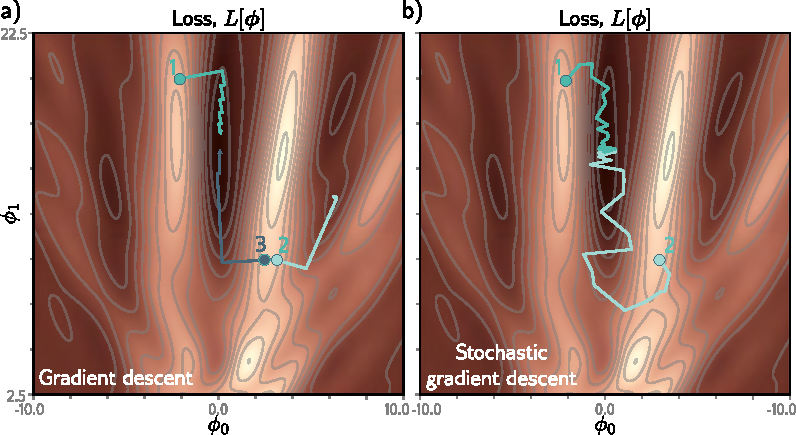
\includegraphics[width=\textwidth]{figures/Intro/sgd.pdf}
    \caption{\textbf{Gradient descent and Stochastic gradient descent. a)} Depicts the trajectory of the error score in 
     a 2D loss function in case of gradient descent with line search from three different initializations. The 
     algorithm converges to the global minimum when it starts from points 1 and 3 while it fails when it starts from 
     point 2, located outside the valley of the global minimum. \textbf{b)} The same experiment solved with stochastic 
     gradient descent achieves good convergence also when initialized from point 2. Indeed, the ``noise'' introduced 
     by the mini-batches drives the updates outside the wrong valley and allow the convergence to the global minimum. 
    Adapted from \cite{prince2023understanding}}
    \label{fig:sgd}
\end{figure}

\subsection{Backpropagation and automatic differentiation}

At this stage, a crucial question arises: \textbf{how can SGD be efficiently implemented in practice?}
ANNs often involve millions or even billions of parameters $\theta$, thus computing exact derivatives with respect to 
such a large number of variables, for every batch and across multiple epochs, requires highly optimized algorithms 
and hardware acceleration.
Indeed, the practical feasibility of training neural networks was significantly advanced by the seminal work of Rumelhart, 
Hinton, and Williams in 1986 \cite{Backpro_1986}, which introduced the efficient \textit{back-propagation} technique that made 
large-scale training computationally tractable.

Back-propagation bases its principles on the fundamental \textit{chain rule} proposed by Leibniz in 1676 to calculate 
derivatives of function compositions. In fact, a ANNs can be seen as a composition of functions (the layers) in which 
at each stage the layer $i$-th processes the output of the layer $(i-1)$-th. Formally, one can write: 

\begin{equation}
    \mathcal{N}_{\theta} = f_\theta^{(L)} \circ f_\theta^{(L-1)} \circ ... \circ f_\theta^{0}
    \label{eq:composition}
\end{equation}

Where $f_\theta^{(L)}$ is the function representing the $L$-th layer of neurons of parameters $\theta$. The gradient 
of the loss function with respect to the parameters is therefore expressed, according to the chain rule as: 

\begin{equation}
    \nabla_{\theta^{(l)}} L  = \frac{\partial{(L)}}{\partial{f^{(L)}}} \cdot \frac{\partial{f^{(L)}}}{\partial{f^{(L-1)}}} 
    \cdot ... \cdot \frac{\partial{f^{(l)}}}{\partial{\theta^{(l)}}}
    \label{eq:chain_rule}
\end{equation}

This method decomposes the calculation of the full gradient into a sequence of smaller, local derivatives, each 
associated with the intermediate states of the network. During the forward pass, the activations and local 
Jacobians are computed and stored in memory, a process sometimes referred to as \textit{forward accumulation}. 
These stored quantities are then systematically reused during the backward pass to propagate gradients from the 
output layer back through the network parameters. This reuse of intermediate computations is what makes the 
algorithm highly efficient, and it is from this backward flow of gradients that the name \textit{back-propagation} 
originates.  

In modern machine learning frameworks such as PyTorch \cite{paszke2019pytorch} and TensorFlow 
\cite{abadi2016tensorflow}, back-propagation is implemented through the construction of a 
\textit{computational graph}. Each node in the graph represents an operation, while edges encode the dependencies 
between operations. Once the forward pass has been executed, this graph allows the backward pass to be automatically 
derived and executed, efficiently parallelized across GPUs or TPUs. In fact, back-propagation is a specific instance 
of a more general family of techniques known as \textit{automatic differentiation} (or \textit{algorithmic 
differentiation}) (AD) \cite{Griewank2000EvaluatingD, baydin2018}, and more precisely corresponds to 
\textit{reverse-mode automatic differentiation}. This connection highlights that back-propagation is not 
unique to neural networks, but rather belongs to rigorous and general framework for computing exact 
derivatives of functions defined by computer programs.  

% It is useful to contrast automatic differentiation with two other approaches for computing derivatives. 
% \textit{Symbolic differentiation}, as implemented for instance in computer algebra systems, manipulates expressions 
% analytically but suffers from expression swell and is not well suited for large computational graphs. 
% \textit{Numerical differentiation}, based on finite-difference approximations, is conceptually simple but prone to 
% numerical instability and scales poorly with the number of parameters. In contrast, automatic differentiation 
% combines the exactness of symbolic methods with the efficiency of numerical approaches, making it particularly 
% well suited for large-scale models such as neural networks.  

\begin{figure}[H]
    \centering
    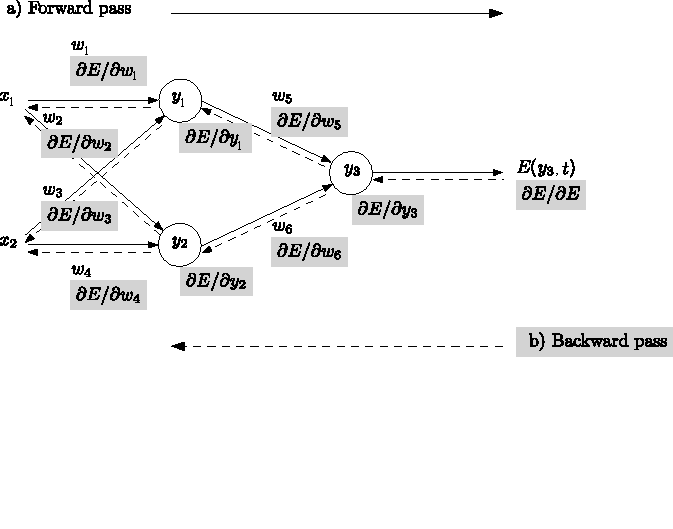
\includegraphics[width=\textwidth]{figures/Intro/backpro.pdf}
    \caption{\textbf{Schematic of Back-propagation on computational graph. a)} The training inputs $x_i$ are processed 
    in the forward pass by the network that produces intermediate states $y_{1,2}$ using weights $w_i$, and the final 
    output $y_3$. \textbf{b)} The error $E$ computed between the output and the estimate $t$ is propagated backward 
    and the gradients with respect to the weights $\nabla_{w_i} E = (\frac{\partial{E}}{\partial{w_1}},..., \frac{\partial{E}}{\partial{w_6}})$
    are obtained from the chain rule of derivatives. Adapted from \cite{baydin2018}}
    \label{fig:sgd}
\end{figure}

\newpage

\section{Convolutional Neural Networks (CNNs)}

It was anticipated earlier in the Chapter that the network design can strongly impact the learning of the mapping 
$\mathcal{M}$. In the specific case in which $\mathcal{X}, \mathcal{Y}$ represent sets of natural images, neural 
networks with layers employing convolution operations have shown to outperform fully connected ones \cite{Fukushima1982,LeCun1989Handwritten, LeCun1989Backpropagation}. 
The reasons behind the success of convolutions are intuitively explained as follows: 

\begin{itemize}

    \item Images are inherently high-dimensional, as they are defined on 2D or 3D grids. As a result, the number of 
    parameters required to connect each pixel in a fully connected neural network grows rapidly and soon becomes 
    intractable. Convolutional layers address this issue by employing a \textit{kernel}: a small trainable filter 
    that is convolved with the input image or intermediate feature maps. This mechanism enables weight reuse across spatial 
    locations, drastically reducing the number of trainable parameters, a property commonly referred to as 
    \textit{parameter sharing}. Furthermore, the localized receptive field of the kernel induces a form of structured 
    sparsity, effectively regularizing the model by constraining the mapping to be approximated using compact, spatially 
    coherent information.

    \item  In images, spatially adjacent pixels are typically correlated, while uncorrelated variations are often 
    attributable to noise. Fully connected layers process each pixel independently, requiring the network to learn 
    spatial dependencies solely through training. Convolutional layers, in contrast, explicitly exploit local spatial 
    correlations by aggregating information from neighboring pixels, thereby embedding structural priors into the 
    architecture. (see Fig. \ref{fig:conv})

    \item The image of a tree and another image of the same tree, translated require a different tuning of the
    weights in a fully-connected layer, although the interpretation of the image has not physically changed. 
    Learning a different parameter configuration for each different translation of the same object is highly inefficient. 
    On the contrary, an additional benefit of the parameter sharing in convolutional layers is the equivariance to 
    translation that inherently optimize the learning. This property allows the output to respond to the input change 
    in the same way. Note that this equivariance is not valid for other geometrical transformations like rotation and 
    magnification.

\end{itemize} 

% motivation
We have seen in Chapter \ref{chap:bcdi} that BCDI data is in the form of 3D images in which peculiar spatial structures 
made of peaks and fringes are clearly visible, hence the natural choice of convolutional neural networks. Moreover, the 
tasks addressed in this PhD thesis, namely the gap-inpainting and the phase retrieval, are classified as inverse problems 
where the goal is to reconstruct missing or unmeasured information from incomplete observations. As highlighted in recent 
surveys and related works \cite{Review_CNN_2020, CNN_inverse2017}, CNNs are particularly well suited for these problems 
because they can learn powerful image priors from data, act as regularizers even without extensive training 
(as shown in the Deep Image Prior framework \cite{Ulyanov_2020}), and can be combined with physics-based models to 
enforce data consistency.

Let us present now the building blocks of a typical convolutional neural network.

\subsection{Convolutional layer}

The initialization of a convolutional layer in typical machine learning libraries involve the definition of: 
\begin{itemize}
    \item An integer number of kernels. This number corresponds to number of filters through which the input is 
    processed in a convolution operation. Each filter is normally associated to a different feature of the input 
    image that is extracted by the corresponding kernel. The output of the convolutional layer will 
    have an extra dimension (called \textit{channel}) with size corresponding to the number of filters.  

    \item The integer-valued size of the kernel. In 2D convolutions the kernel is a matrix and similarly 
    extended to a 3D tensor for three-dimensional inputs. It controls the scale of the features that the convolutional 
    layer can ``see''. Small kernels highlight small features and vice-versa.

    \item The padding parameter which handles the convolution at the borders of the image, where the kernel would 
    otherwise extend beyond the available data. It determines whether the output feature map maintains the same spatial 
    dimensions as the input (``same'' padding) or is reduced in size (``valid'' padding).

    \item The stride parameter: This integer-valued parameter (matrix in 2D and tensor in 3D) indicates the lateral shift 
    that is applied to the kernel across the image. If greater than 1 some pixels/voxels are skipped resulting in a 
    sort of sub-sampling allowing to filter out some low-level features. 
    
    \item The dilation rate, which is another integer-valued parameter (matrix in 2D and tensor in 3D) that allows 
    to insert holes between consecutive elements of the kernel. In this way the actual size of the kernel is increased 
    by the dilation value, but the overall number of weights is unvaried. This enables to cover a larger area of the input 
    without increasing the number of trainable parameters.

\end{itemize}

Additional features of a typical convolutional layer include the addition of trainable biases and the initialization and 
regularization of the kernels and biases. Lastly, a non-linear activation is usually applied to the output of 
the convolutional layer. 

We mention here the existence of so-called \textit{transposed convolutions} which are sometimes used in CNNs. Here the 
conceptual difference is that instead of sliding the kernel over the input, is the input sliding over the kernel and 
performing the element-wise multiplication and summation. Transposed convolutions naturally produce an output that is larger 
than the input, because they reverse the spatial reduction of a standard convolution. For this reason, they are often used 
to replace explicit \textit{up-sampling} layers, which increase the spatial size through fixed interpolation (e.g. nearest-
neighbor or bilinear). Unlike standard interpolation, transposed convolutions perform a \textit{learned} up-sampling, 
where the network optimizes the kernel weights to reconstruct high-resolution features in a data-driven way. 

\begin{figure}[H]
    \centering
    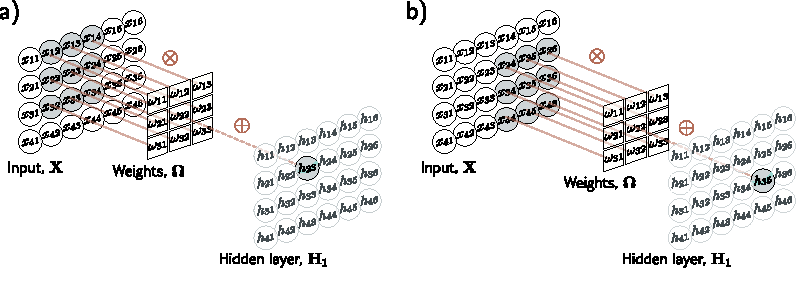
\includegraphics[width=\textwidth]{figures/Intro/conv.pdf}
    \caption{\textbf{Schematic of 2D convolutional layer:  a) } The convolution is operated over a region of the image 
    with same size as the kernel ($3 \times 3$). The result of the multiplication of each pixel value $(x_{12},...,x_{34})$ 
    times the weight $(w_{11},...,w_{33})$ is then summed into a scalar $h_{23}$. \textbf{b)} The same operation with 
    the same kernel is performed to a shifted window of the input image.
    Adapted from \cite{prince2023understanding}}
    \label{fig:conv}
\end{figure}

\subsection{Pooling Layer}

After the convolutional layer and the activation function, it is often the turn of a \textit{pooling} layer. For the 2D case, 
the output of the layer at specific location $i,j$ is the result of a filtering operation on the neighboring pixels 
of the input. For instance, the ``Max Pooling'' layer replaces a rectangular region of the input with its maximum value, 
thus retaining only the strongest activation within that area. In contrast, the ``Average Pooling'' layer 
assigns to the output pixel the mean value of all pixels in the corresponding region. 
The benefits deriving from the pooling layer are mostly twofold. First, the size of the output is reduced by a factor 
proportional to the area of the pooling window (or the volume in the 3D case), thus lowering the computational 
and memory cost of subsequent operations. Second, by condensing information into a smaller region, pooling encourages 
the network to learn representations that are more robust to small translations. For instance, with Max Pooling, 
a shift of the most activated pixel within the pooling window does not affect the output. This behavior can be 
interpreted as an implicit prior that biases the optimization towards translation-invariant approximations. 

\begin{figure}[H]
    \centering
    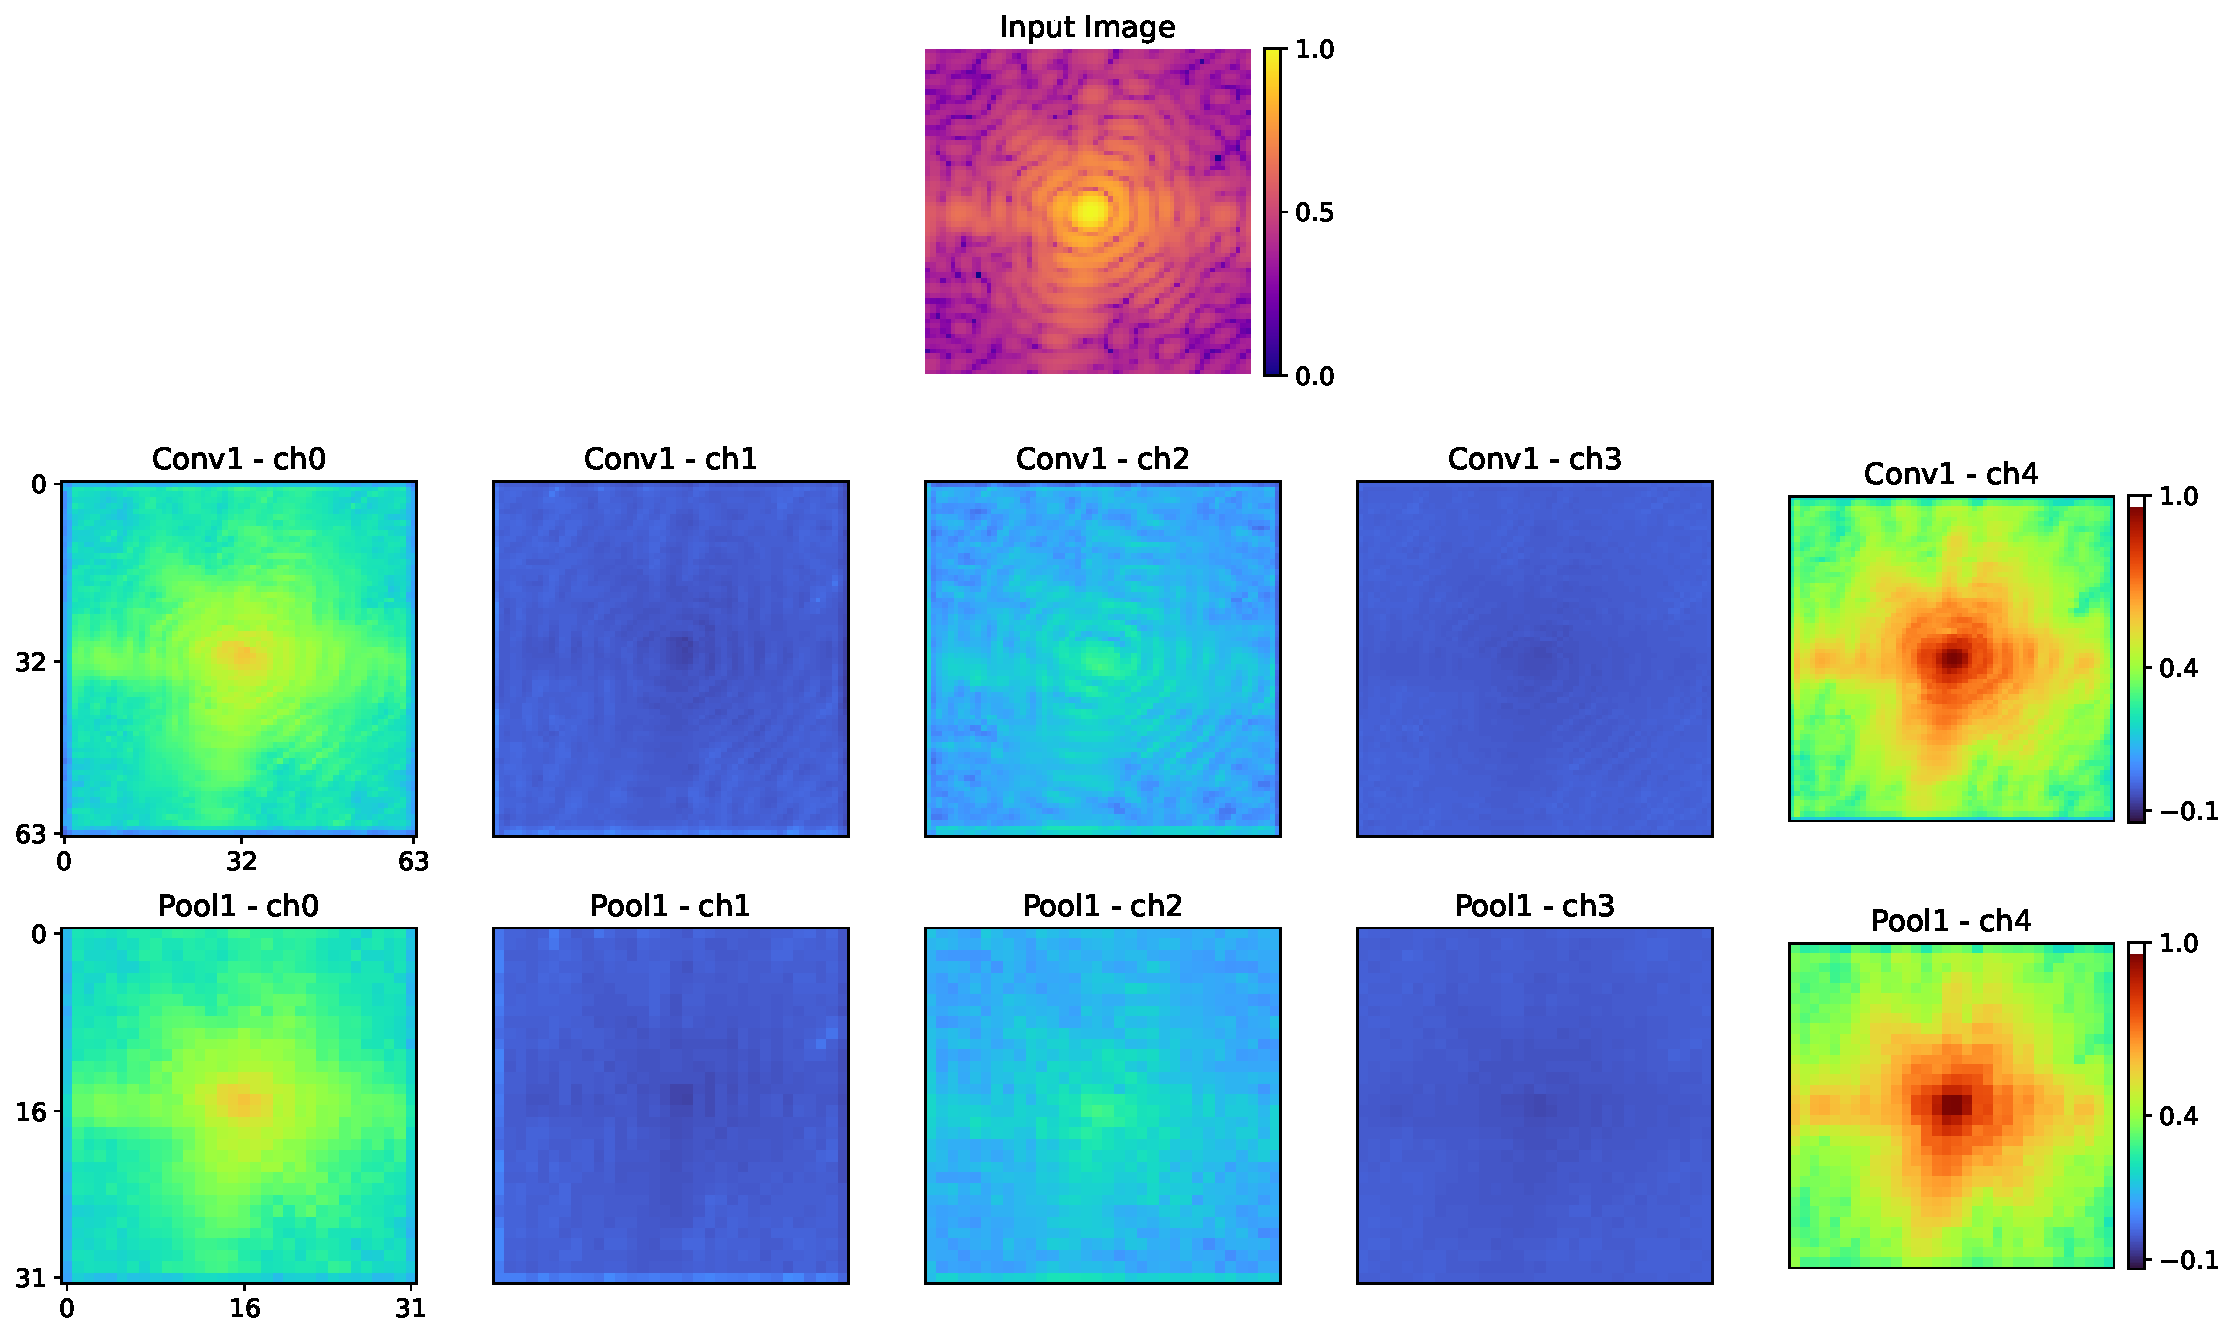
\includegraphics[width=\textwidth]{figures/Intro/conv_maxpool.pdf}
    \caption{\textbf{Example of Convolutional and Max pooling layers.} A simulated 2D BCDI pattern is input image 
    (first row) of the CNN model presented later in Chapter \ref{chap:phase_retrieval}, after the training. The output of the first 
    convolutional layer + LeakyReLU activation is displayed in the second row (first 5 channels) while the output of 
    the subsequent Max Pooling layer is displayed in the third row. Notice the similarity between the two rows despite 
    the halved size of Max Pooling output. This shows that it efficiently condenses the information into smaller sizes.
    % Moreover, one can notice how different channels extract different features, some of which (0 and 4 in this case) 
    % have larger amplitude, thus ``importance'' to the network.
    }
    \label{fig:convmaxpool}
\end{figure}


The typical convolutional block is therefore composed of these three layers (convolutional, activation, pooling). 
A sequential application of the convolutional blocks to a 2D or 3D input image is often called \textit{encoder} and 
can reduce the dimension of the 
feature map to as many 1D vectors as the number of filters of the last convolutional layer. During the training, this 
reduced representation of the input is more and more driven to capture the essential information in a lower-dimensional 
space. At this point, for \textit{classification} tasks the feature map is flattened into a single 1D vector 
being the input of a fully connected layer. The output of this last layer is then usually interpreted as the probability 
score for the input image to belong to a specific class. Among the milestone CNN models for classification, it is worth 
highlighting LeNet-5, introduced by LeCun in 1998 \cite{lecun1998gradient}, and AlexNet, which revolutionized the 
field by leveraging more efficient GPU-based training \cite{krizhevsky2012imagenet}.

In \textit{image generation} tasks, the lower-dimensional space, also called \textit{latent space} serves as input 
to a sequence of 
\textit{deconvolutional} blocks, where \textit{transposed} convolutions combined with activation functions 
progressively reconstruct the output image at the desired resolution. This sequence of deconvolutional layers 
is referred to as the \textit{decoder}, as it mirrors the encoder. In some architectures, up-sampling layers 
followed by standard convolutions are employed instead of transposed convolutions. Encoder-decoder architectures 
for image generation were first introduced by Hinton in 2006~\cite{hinton2006reducing}. This class of models is employed 
in a variety of tasks such as de-noising, image compression, inpainting, 
and segmentation. Although other types of models are also used for image generation, including Generative 
Adversarial Networks (GANs) \cite{goodfellow2014generativeadversarialnetworks} and Vision Transformers 
(ViTs) \cite{dosovitskiy2021imageworth16x16words}, in this manuscript we restrict our focus to 
encoder-decoder architectures.


\subsection{Skip connections}

Before concluding the chapter it is worth mentioning the concept of \textit{skip connections} (or \textit{residual 
connections}). 
